\documentclass{beamer}

\usepackage[utf8]{inputenc}
\usepackage[greek,english]{babel}
\usepackage{alphabeta}
\usepackage{amsmath}
\usepackage{graphicx}
\usepackage{hyperref}
\usepackage{xcolor}
\usepackage[dvipsnames]{xcolor}

\hypersetup{colorlinks=true, linkcolor=black, urlcolor=black, citecolor=black}

\title{EchoLite: Υλοποίηση Συστήματος Μέτρησης Απόστασης με Υπερηχητικό Αισθητήρα σε FPGA Χρησιμοποιώντας VHDL}
\author{Ιορδάνης Κωστελίδης}
\date{18/06/2025}
\institute{Πρόγραμμα Μεταπτυχιακών Σπουδών στη Ρομποτική \\
Τμήμα Μηχανικών Πληροφορικής, Υπολογιστών και Τηλεπικοινωνιών \\
Πολυτεχνική Σχολή \\
Διεθνές Πανεπιστήμιο της Ελλάδος}

\begin{document}

\begin{frame}
  \titlepage
\end{frame}

\begin{frame}{Εκφώνηση Εργασίας}
\begin{itemize}
  \item Σχεδιασμός κυκλώματος σε VHDL για την πλακέτα \textbf{DE10-Lite}
  \item Χρήση υπερηχητικού αισθητήρα \textbf{HC-SR04} για μέτρηση απόστασης
  \item Απεικόνιση απόστασης σε \textbf{7-segment displays}
  \item Προαιρετικά: σχεδίαση εξωτερικού κυκλώματος σε KiCad
\end{itemize}
\end{frame}

\begin{frame}{Επισκόπηση του Έργου}
\begin{itemize}
  \item Υλοποιήθηκε πλήρως σε \textbf{VHDL} χωρίς χρήση μικροελεγκτή
  \item Πραγματοποιείται μέτρηση απόστασης σε \textbf{πραγματικό χρόνο}
  \item Η έξοδος προβάλλεται σε \textbf{δύο 7-segment displays}
  \item Σχεδιάστηκε και το \textbf{εξωτερικό κύκλωμα σε KiCad}, αλλά δεν εγινε παραγγελία λόγω χρόνου
\end{itemize}
\end{frame}

\begin{frame}{Λίστα Υλικών}
\begin{itemize}
  \item FPGA: \textbf{DE10-Lite} με Altera MAX 10
  \item Υπερηχητικός αισθητήρας: \textbf{HC-SR04}
  \item Καλώδια σύνδεσης και breadboard
  \item Software: Windows 11 Pro*, Quartus Prime Lite Edition, QuestaIntel Starter FPGA Edition, KiCad
\end{itemize}
\end{frame}

\begin{frame}{Αρχιτεκτονική Συστήματος}
\begin{itemize}
  \item \textbf{MHzClock}: μετατροπή 50MHz σε 1MHz
  \item \textbf{HCSR04}: διαχείριση αισθητήρα \& υπολογισμός απόστασης
  \item \textbf{SevenSegmentDisplay}: εμφάνιση δεκαδικού αριθμού 1 ψηφίου
  \item \textbf{Multi-SevenSegmentDisplay}: εμφάνιση δεκαδικού αριθμού 2 ψηφίων
\end{itemize}
\end{frame}

\begin{frame}
\frametitle{Διάγραμμα}
	\centerline{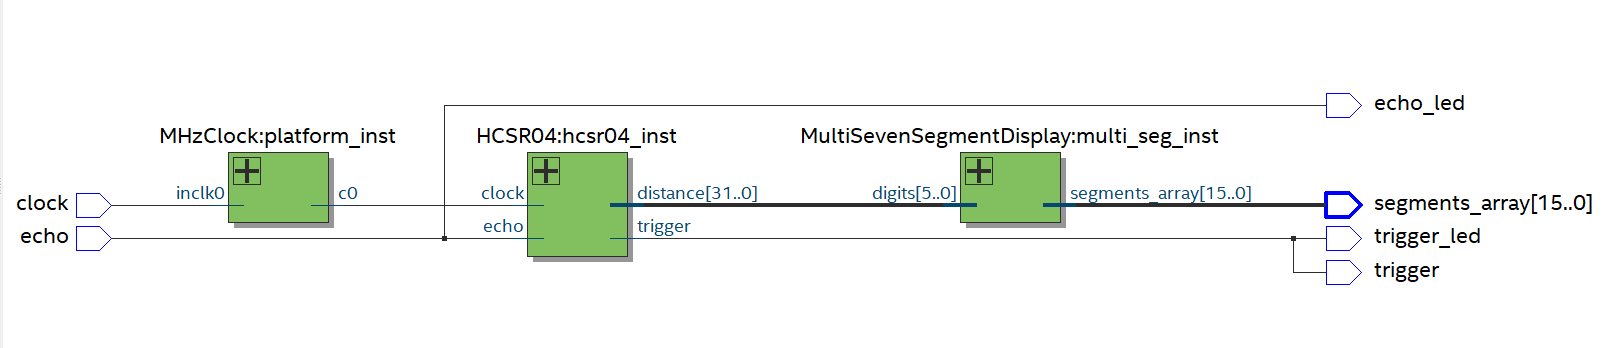
\includegraphics[width=1\textwidth]{assets/echolite.png}}
\end{frame}

\begin{frame}{HCSR04}
\begin{itemize}
  \item Παλμός \textbf{trigger} διάρκειας 10 μικροδευτερολέπτων
  \item Μέτρηση διάρκειας του \textbf{echo} παλμού
  \item Υπολογισμός απόστασης με βάση $\text{distance} = \frac{techo \cdot 0.0343}{2}$
  \item Στο VHDL: $\text{distance} \approx techo \cdot 17 / 1000$
\end{itemize}
\end{frame}

\begin{frame}
\frametitle{Simulation}
	\centerline{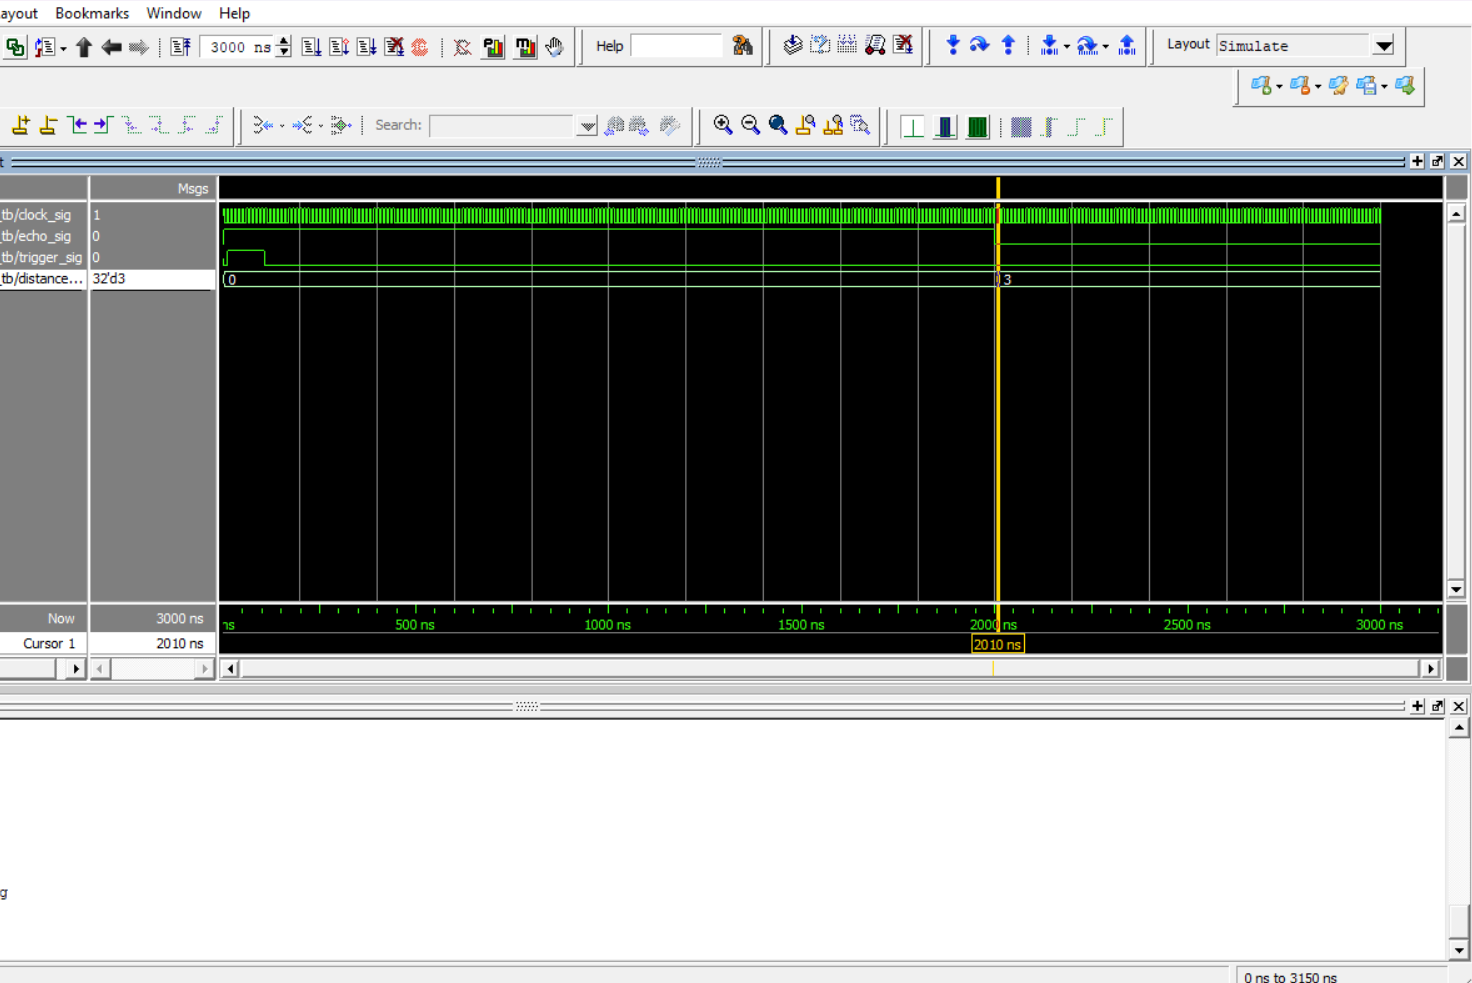
\includegraphics[width=1\textwidth]{assets/hcsr04-tb.png}}
\end{frame}

\begin{frame}{SevenSegmentDisplay}
\begin{itemize}
  \item Προβολή 1 ψηφίου από δυαδική είσοδο 4-bit
  \item Μετατροπή αριθμού σε κωδικοποίηση για LED segments
  \item Υποστήριξη ψηφίων 0–9 με χρήση \texttt{CASE} statement
\end{itemize}
\end{frame}

\begin{frame}
\frametitle{Προσομοίωση}
	\centerline{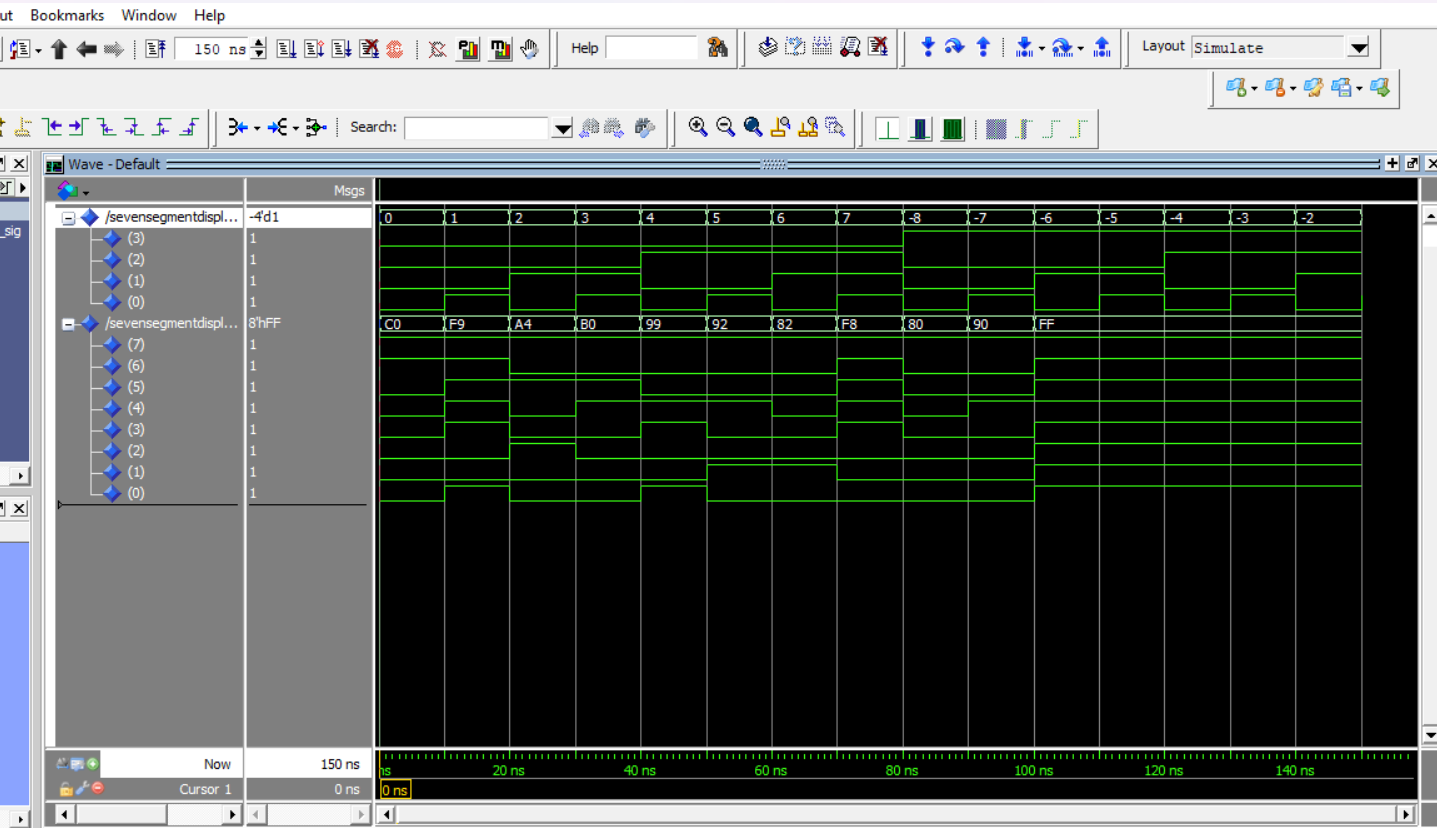
\includegraphics[width=1\textwidth]{assets/ssd-tb.png}}
\end{frame}

\begin{frame}
\frametitle{Πραγματικό}
	\centerline{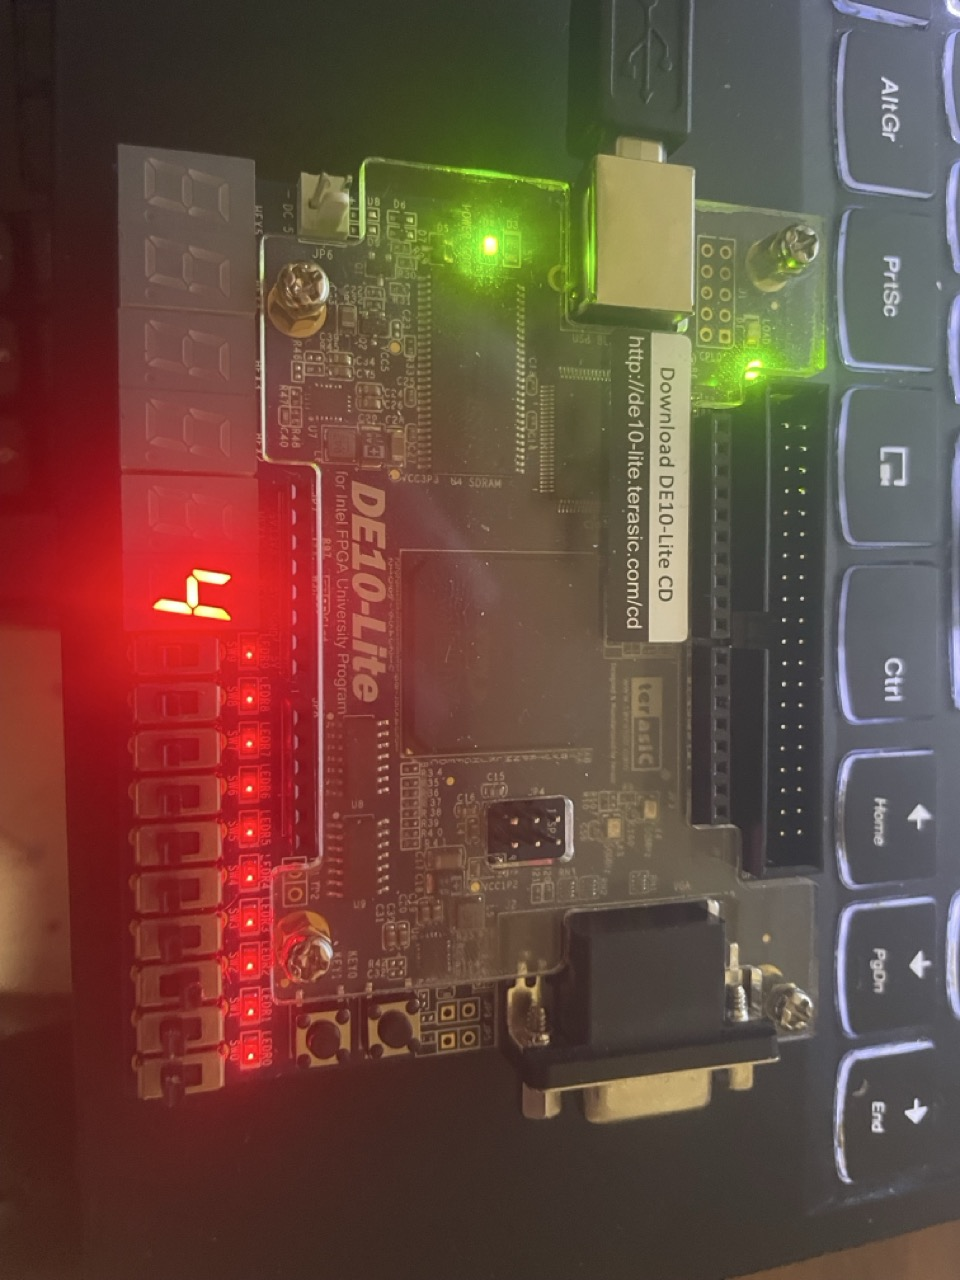
\includegraphics[angle=90, width=1\textwidth]{assets/ssd-real.jpeg}}
\end{frame}

\begin{frame}{Multi Seven Segment Display}
\begin{itemize}
  \item Μετατροπή 6-bit αριθμού σε δύο δεκαδικά ψηφία
  \item Χρήση πίνακα για τον χειρισμό πολλών 7-segment
  \item Επαναχρησιμοποίηση της μονάδας 1-ψηφίου
\end{itemize}
\end{frame}

\begin{frame}
\frametitle{Προσομοίωση}
	\centerline{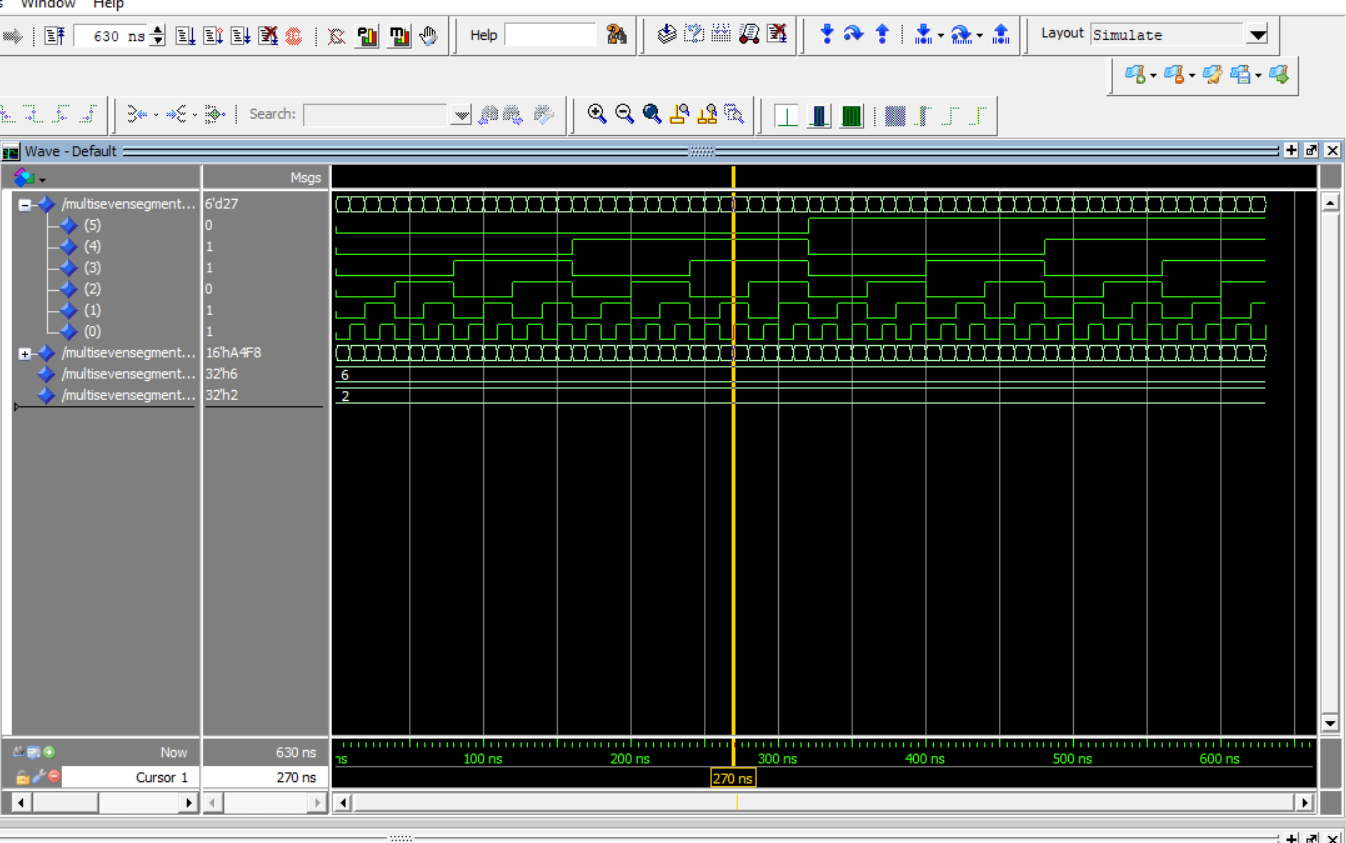
\includegraphics[width=1\textwidth]{assets/mssd-tb.png}}
\end{frame}

\begin{frame}
\frametitle{Πραγματικό}
	\centerline{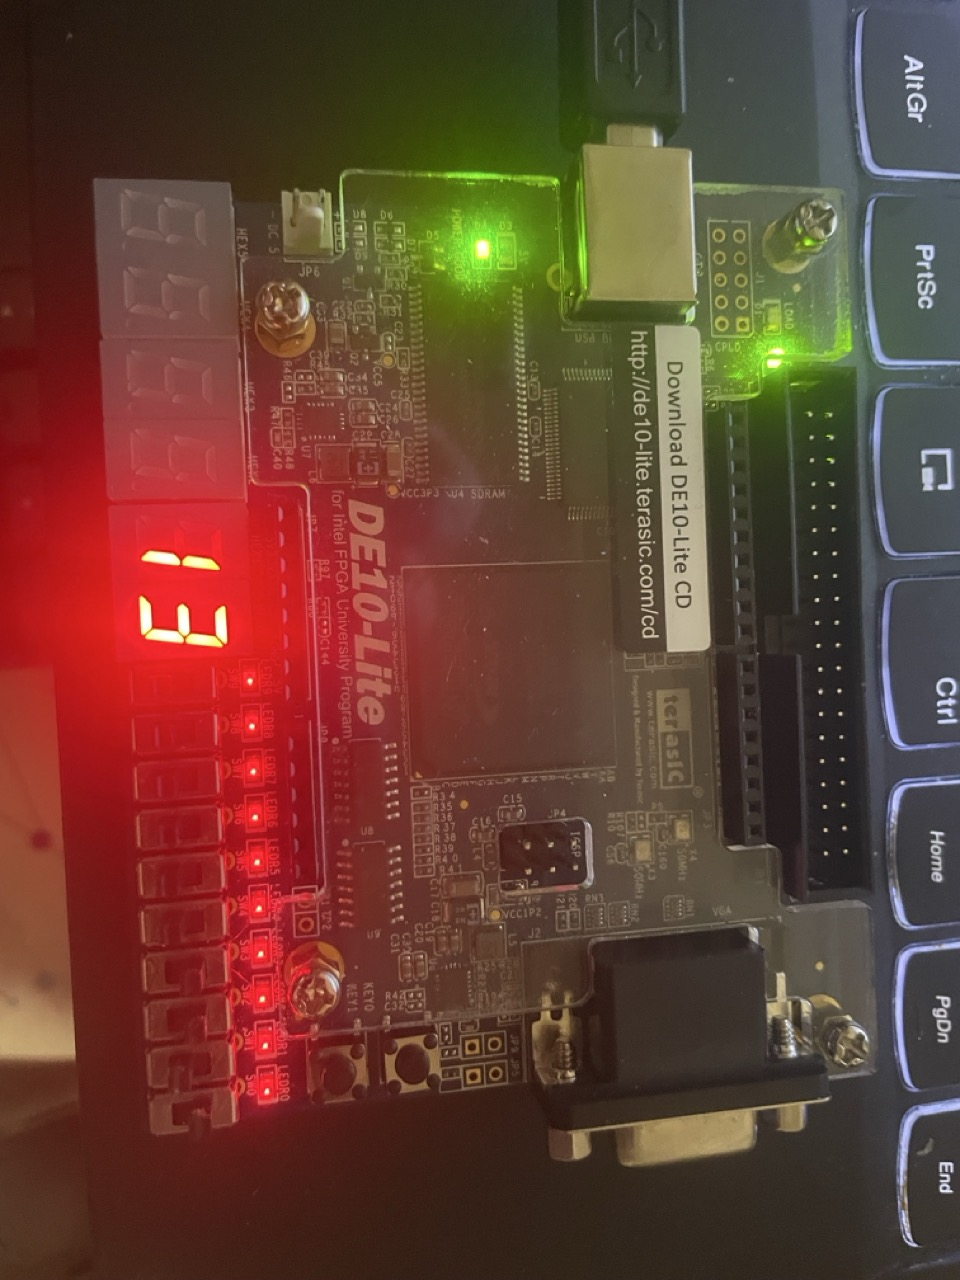
\includegraphics[angle=90, width=1\textwidth]{assets/mssd-real.jpeg}}
\end{frame}

\begin{frame}{EchoLite}
\begin{itemize}
  \item Ενσωμάτωση όλων των υπομονάδων σε ενιαίο σύστημα
  \item Ενδείξεις απόστασης: 2 ψηφία σε 7-segment
  \item Έλεγχος συγχρονισμού και ρολογιού με ALTPLL
\end{itemize}
\end{frame}

\begin{frame}
\frametitle{Πραγματικό}
	\centerline{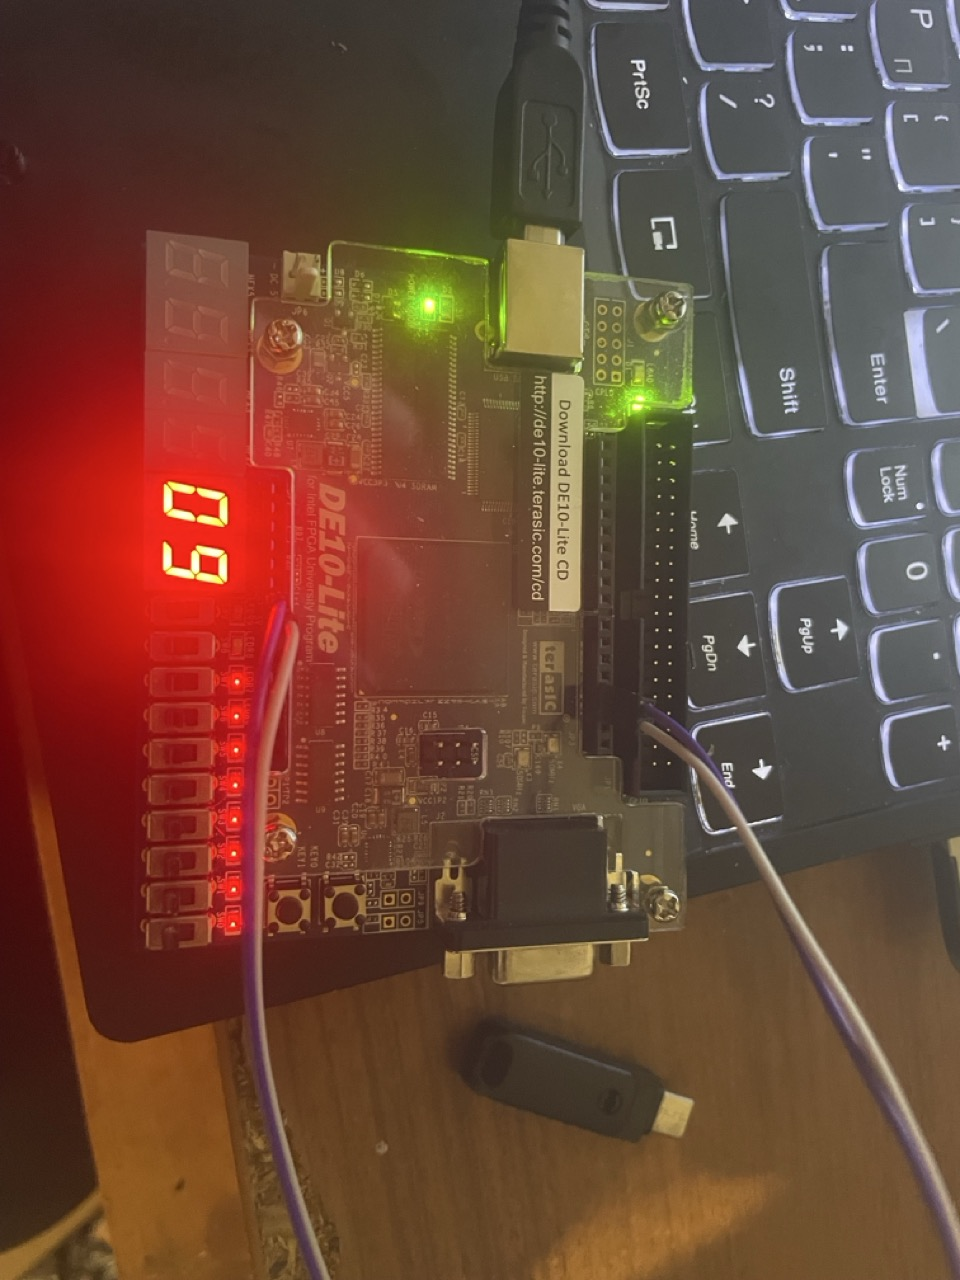
\includegraphics[angle=90, width=1\textwidth]{assets/echolite-real.jpeg}}
\end{frame}

\begin{frame}
\frametitle{Live Demo}
	Live Demo
\end{frame}

\begin{frame}{Πόροι Υλοποίησης}
\begin{itemize}
  \item Logic Elements: 984
  \item Registers: 104
  \item I/O Pins: 21
  \item PLLs: 1 (ALTPLL για δημιουργία 1MHz ρολογιού)
\end{itemize}
\end{frame}

\begin{frame}{Δοκιμές και Αποτελέσματα}
\begin{itemize}
  \item Επιτυχής μέτρηση αποστάσεων σε πραγματικό χρόνο
  \item Έλεγχος βασικών μονάδων με test benches
  \item Πραγματικές μετρήσεις με χρήση DE10-Lite
\end{itemize}
\end{frame}

\begin{frame}{Σχεδίαση PCB}
\begin{itemize}
  \item Custom πλακέτα
  \item Arduino Uno R3 Shield
  \item HC-SR04
\end{itemize}
\end{frame}

\begin{frame}
\frametitle{Schematic}
	\centerline{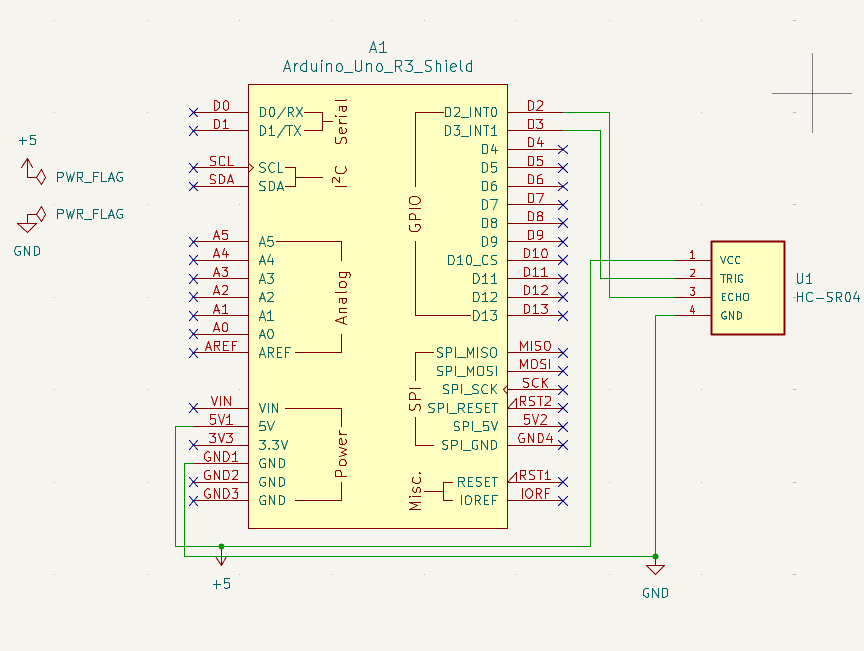
\includegraphics[width=1\textwidth]{assets/schematic.png}}
\end{frame}

\begin{frame}
\frametitle{PCB}
	\centerline{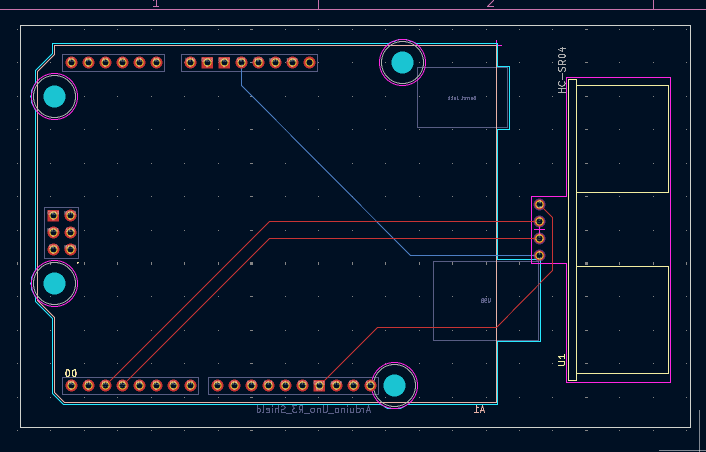
\includegraphics[width=1\textwidth]{assets/pcb.png}}
\end{frame}

\begin{frame}
\frametitle{PCB 3D}
	\centerline{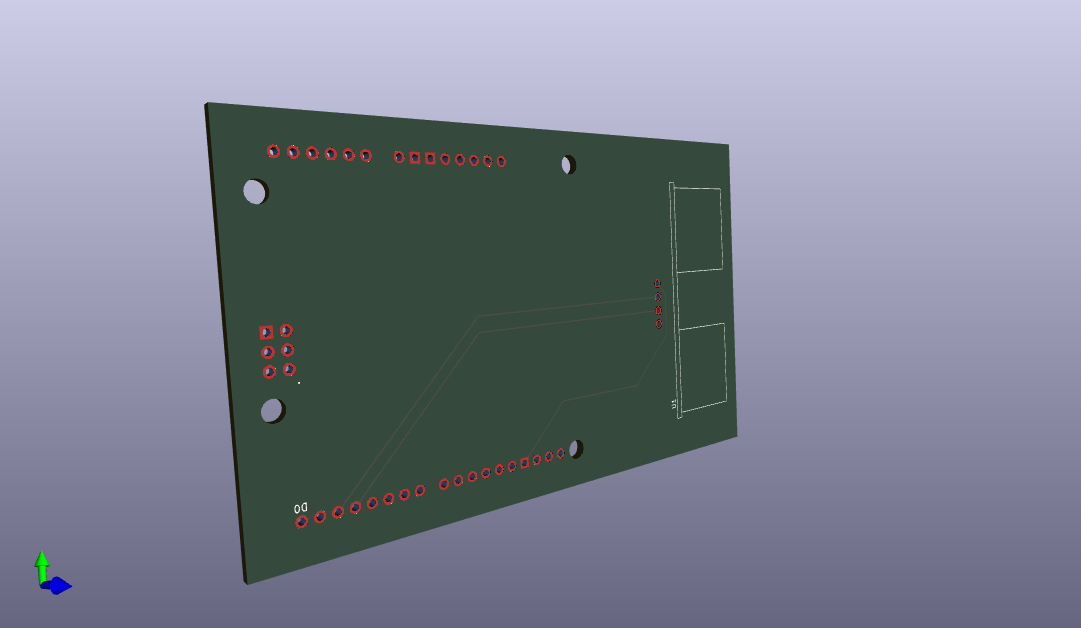
\includegraphics[width=1\textwidth]{assets/pcb-3d.png}}
\end{frame}

\begin{frame}{Μελλοντική Εργασία}
\begin{itemize}
  \item Παραγγελία, συναρμολόγηση και δοκιμή της πλακέτας
  \item Υποστήριξη περισσότερων 7-segment (π.χ. 3 ψηφία) ή LCD
\end{itemize}
\end{frame}

\begin{frame}{Κώδικας και σχετικά}
\centering
\begin{itemize}
  \item http://github.com/KostelidisDev/EchoLite
\end{itemize}
\end{frame}

\begin{frame}{Ερωτήσεις \& Ευχαριστίες}
\centering
Ευχαριστώ πολύ! \\ Μπορείτε να θέσετε ερωτήσεις.
\end{frame}

\end{document}